\chapter{AmaaS - Atomic Multicast as a Service}\label{ch:amaas}

% **************************** Define Graphics Path **************************
    \graphicspath{{Chapter3-TxService/Figs/Vector/}{Chapter3-TxService/Figs/}}

This chapter introduces the concept of providing \emph{amcast} messaging as a service to members of a cluster.

First we describe the rationale behind \textsf{Amaas}, then we explore the requirements of such a service and the challenges involved in meeting them.  This is followed by the introduction of \textsf{SCast} - an \emph{amcast} protocol that utilises the \textsf{AmaaS} model.  Finally, we discuss the limitations of existing \emph{abcast} protocols in the context of an \textsf{AmaaS} ordering service, and propose the need for a new non-blocking \emph{abcast} solution.  

\section{Rationale}
Total order commit protocols can be utilised by distributed systems to coordinate transactions without the use of locks.  They reduce the abort rate of transactions when contention is high, as system deadlocks cannot occur when distributed locks are not present.  Therefore, they can aid scalability and improve transaction throughput \citep{Ruivo:2011:ETO:2120967.2121604}.  

The limiting factor of a total order commit protocol is the underlying mechanism used to provide atomic guarantees on message delivery.  For example, the \emph{amcast} protocol, TOA, currently utilised by Infinispan, does not scale well as the number of destinations $N$ increase, as $N->1$ communication is expensive ($\S$ \ref{ssec:TOA_limations}).  Similarly, other GM protocols such as Newtop \citep{Ezhilchelvan:1995:NFG:876885.880005}, exasperate the problem, as the number of messages required to perform an \emph{amcast} increases dramatically as $N$ increases.  Finally, quorum-based protocols provide even less scalability, then GM based protocols, as their inability to \emph{amcast} messages to disjoint sets of nodes typically requires all nodes in the cluster to participate in an \emph{abcast}.  

As the atomic multicast protocols required by the total order commit protocol are inherently unscalable, we argue that transaction coordinators should not be burdened with the responsibility of reaching a consensus on transaction ordering.  We propose that transaction ordering should not be conducted between the transaction coordinator and the Infinispan nodes participating in the transaction, rather transaction ordering should be provided by an independent ordering service.  This decoupling of ordering and transactions, allows the transaction coordinator to request and receive a total order from the service, before multicasting its $prepare(Tx)$ message to all nodes participating in the transaction.  Such an approach results in the number of nodes involved in a transaction having no effect on the total number of nodes participating in consensus, instead the number of nodes in a transaction only increases the number of unicasts required when sending the transaction's $prepare(Tx)$ message \footnote{Such a cost is unavoidable as the number of destinations will always determine the minimum number of unicasts required to disseminate a $prepare(Tx)$ message.}.  

The most efficient implementation of such an ordering service, in terms of latency, would consist of a single node providing transaction ordering to all Infinispan nodes.  However, as the progress of all Infinispan transactions is dependent on this ordering service, it is necessary for crash-tolerance to be provided.  Therefore, we envisage such a service consisting of a dedicated set of nodes which act as a single state machine, with consensus being required amongst all nodes within the service, when a new ordering request is received from an Infinispan transaction.  Hence, such an approach limits the number of nodes required to reach a consensus on ordering to the total number of nodes providing the ordering service, regardless of the number of nodes involved in a transaction.  

We call this system model Atomic Multicast as a Service (\textsf{AmaaS}), and refer to the existing Infinispan approach as \emph{peer-to-peer} (P2P).  The next section of this chapter provides a detailed description of this system model.    	

\section{System Model}	
	The \textsf{AmaaS} approach introduces the concept of a dedicated set of nodes providing ordering to another disjoint set of nodes whom participate in distributed transactions.  We define the nodes providing the ordering service as service nodes, $s$-nodes for short, and denote them as $N_s1 \ldots N_sn$, where $n \geq 2$.  As we consider a crash-tolerant ordering service essential, we do not consider $n = 1$.  We refer to the consumers of this ordering service as client nodes, or $c$-nodes for short, and denote them as $N_c1 \ldots$ $N_cx$; where $x$ is the total number of $c$-nodes utilising the ordering service.  
		
    For all unicasts sent between correct nodes, we assume that messages are sent via a reliable network protocol, such as TCP\citep{Cerf:2005:PPN:1064413.1064423} or Reliable UDP\citep{ReliableUDP}, and they arrive within an unknown delay bound.   Furthermore, all references to a message being \emph{multicast} assumes that the message is unicast to all of the destinations in the message's destination set.  Therefore, if all unicasts between correct nodes are guaranteed to be received, it is also guaranteed that all multicast messages sent between correct nodes will eventually be received by all destinations.  
		
    In our system model we assume that any node, both $s$-nodes and $c$-nodes, can crash at any time, however we do not consider other types of node failures such as byzantine failures.  In order to detect node crashes we assume that a GM service and associated failure detection protocols, such as the ones detailed in section \ref{ssec:jgroups_gms}, are utilised by both service and client nodes.  We assume that a node crash will eventually be detected by the GM service and an updated view of the current network will be received by all nodes once the GM service has detected the crash; hence all nodes within the current view will eventually know of a crash and receive a new view.  Furthermore, we assume that client and service nodes utilise their own GM service, as it is envisaged that the service will operate independently of the client nodes.  Therefore, if an $s$-node crashes, only $s$-nodes will receive a new view, with clients only becoming aware of the $s$-node crash when they interact with the ordering service.  Similarly, if a $c$-node crashes, only $c$-nodes will receive a new view.  Finally, we assume that the GM services employed by the two sets of nodes does not falsely suspect a node of crashing, as the probability of such an event occurring is close to zero as detailed in section \ref{ssec:jgroups_gms}.  
    
	
\section{AmaaS Requirements}\label{sec:absaas_requirements}
The \textsf{AmaaS} model consists of two distinct entities: $s$-nodes and $c$-nodes.  This section will explore the requirements that need to be met in order for the \textsf{AmaaS} model to be effective.  We consider requirements from the perspective of both client and service nodes.

	\subsection*{Client Requirements}
	\begin{itemize}
		\item [\textbf{CR1}] A $c$-node must be able to send \emph{amcast}s to multiple destination sets that may overlap.
		
		\item [\textbf{CR2}] A $c$-node should be able to submits its \emph{amcast} requests to any one of the correct $s$-nodes.  
		
		\item [\textbf{CR3}] Upon receiving \emph{amcast} $m_j$ via the ordering service, a $c$-node must be able to deduce every $m_i$ that is ordered before $m_j$ and has itself as a multicast destination:
		\begin{equation*}
		    \mbox{all}\; m_i : \quad c\mbox{-node} \in m_i.dst \cap m_j.dst \;\mbox{\underline{and}}\; m_i \;\mbox{is ordered before}\; m_j
		\end{equation*}
	\end{itemize}
	
    \subsection*{Service Requirements}
	\begin{itemize}
		\item [\textbf{S1}] The service must provide crash-tolerance ($|s\text{-nodes}| > 1$).
		
		\item [\textbf{S2}] The service must be highly available and non-blocking in the event of an $s$-node crashing or being suspected of having crashed.  
				
		\item [\textbf{S3}] All $s$-nodes must process client requests in the exact same order.
		
		\item [\textbf{S4}] All $s$-nodes should be able to handle client requests.  %, to allow for high availability and to prevent a single $s$-node becoming a performance bottleneck.
	\end{itemize}

\section{SCast: Atomic Multicast Protocol for AmaaS}\label{sec:scast_protocol}
We have developed a protocol for the \textsf{AmaaS} model, which we call \textsf{SCast}; as the protocol offers atomic ordering for multicast messages as a service, hence Service Multicast - \textsf{SCast}.  The \textsf{SCast} protocol enables atomic multicasting by $c$-nodes utilising an ordering service, precisely defining the interactions required between $c$-nodes and the ordering service in order to ensure the atomicity of each multicast.  

Inside the ordering service, the \textsf{SCast} protocol maintains a replicated state machine amongst $s$-nodes that stores the total order timestamps attributed to $c$-node requests.  \textsf{SCast}'s ability to meet requirements S1 - S3, is dependant on the characteristics of this underlying \emph{abcast} protocol utilised  for state machine replication between $s$-nodes, with only S4 guaranteed regardless of the \emph{abcast} protocol used \footnote{This can be guaranteed even if a leader based \emph{abcast} protocol is utilised, as client requests can simply be forwarded to the leader node.  Such an approach can be seen in both Chubby and Zookeeper}.  For example, consider requirement S2.  If the underlying \emph{abcast} protocol is GM based, then message delivery will block in the event of a node crash, therefore it is not possible for S2 to be met with a GM based protocol as the $s$-nodes will become blocked if an $s$-node fails.  Ultimately the performance and \emph{liveness} of an ordering service implementing \textsf{SCast} is tightly coupled to that of the underlying \emph{abcast} protocol which is utilised for state machine replication between $s$-nodes.  

As \textsf{SCast} defines how $c$-nodes interact with the ordering service and how $s$-nodes maintain a replicated state, it is necessary for the protocol to be explained from the perspective of both client and service nodes.  In the explanations below we assume that Infinispan is executing a 1-Phase Total Order transaction, without a second WSC phase, and that the transaction has already been successfully executed locally.  Finally, we refer to a collection of $s$-nodes providing the \emph{amcast} service as the \emph{ordering service}.  
    
    \subsection{Protocol Overview}    
        \subsubsection*{Client Nodes}
    Stage 1 of the client \textsf{SCast} protocol starts once a transaction coordinator, $Tx_i.c$, has completed its local execution of $Tx_i$ and it is ready to \emph{amcast} a $prepare(Tx_i)$ message to $Tx_i.dst$ as required by the total order commit protocol.  The key stages of the \textsf{SCast} protocol from the perspective of a client node are detailed below:
    
    \begin{enumerate}
        \item    \textbf{Delegate Backup Coordinator} - Transfer the contents of $Tx_i$ to a backup coordinator.    
        
        \item    \textbf{Request Ordering} - Send an ordering request to the service as $req(Tx_i)$, and wait for a response message $rsp(Tx_i)$.  
        
        \item    \textbf{Receive Ordering} - Receive $rsp(Tx_i)$ and multicast $Tx_i$ with its ordering data to all $d \in Tx_i.dst$ as $mcast(Tx_i)$.  
        
        \item    \textbf{Order Transaction} - Receive $mcast(Tx_i)$ from $Tx_i.c$, before delivering $Tx_i$ locally with respect to its specified place in the total order.   
    \end{enumerate}
    
    Figure \ref{fig:scast_client} illustrates the four key stages of the \textsf{SCast} protocol outlined above.  Note, that for any $d \in Tx_i.dst$, that is not the active $Tx_i.c$, only step 4 of the protocol is required.  The content and significance of the operations $req(Tx_i)$, $rsp(Tx_i)$ and $mcast(Tx_i)$ are discussed in section \ref{ssec:scast_details}.  

    \begin{figure}[htbp!] 
        \centering    
         \includegraphics[width=1.0\textwidth]{scast_client}
         \caption[SCast Client Interactions]{SCast Client Interaction Diagram}
         \label{fig:scast_client}
    \end{figure}	
    
    
    \subsubsection*{Service Nodes}
    Stage 1 of the service protocol starts when an ordering request, $req(Tx_i)$, is received by an $s$-node, $N_s1$.  It is anticipated that each $s$-node will handle many requests simultaneously, however for the sake of brevity our explanations assume that the service is only handling a single request at a given time.  The key stages of the \textsf{SCast} protocol from the perspective of $N_s1$ are detailed below:
    
     \begin{enumerate}
        \item    \textbf{Receive Request} - Receive client request $req(Tx_i)$.
        
        \item    \textbf{Send Atomic Broadcast} - Process $req(Tx_i)$ and \emph{abcast} it to all $s$-nodes in the service, $abcast(Tx_i)$.  
        
        \item    \textbf{Update Ordering Data} - Deliver $abcast(Tx_i)$ locally and update the stored ordering data to include $Tx_i$.  
    
        \item    \textbf{Return Ordering} - Sends a response message, $rsp(Tx_i)$, to $Tx_j.c$, which contains all of the data required by $c$-nodes to order $Tx_i$.  
    \end{enumerate}
    
    Figure \ref{fig:scast_service} illustrates the four key stages of the \textsf{SCast} protocol outlined above.  
    
    \begin{figure}[htbp!] 
        \centering    
         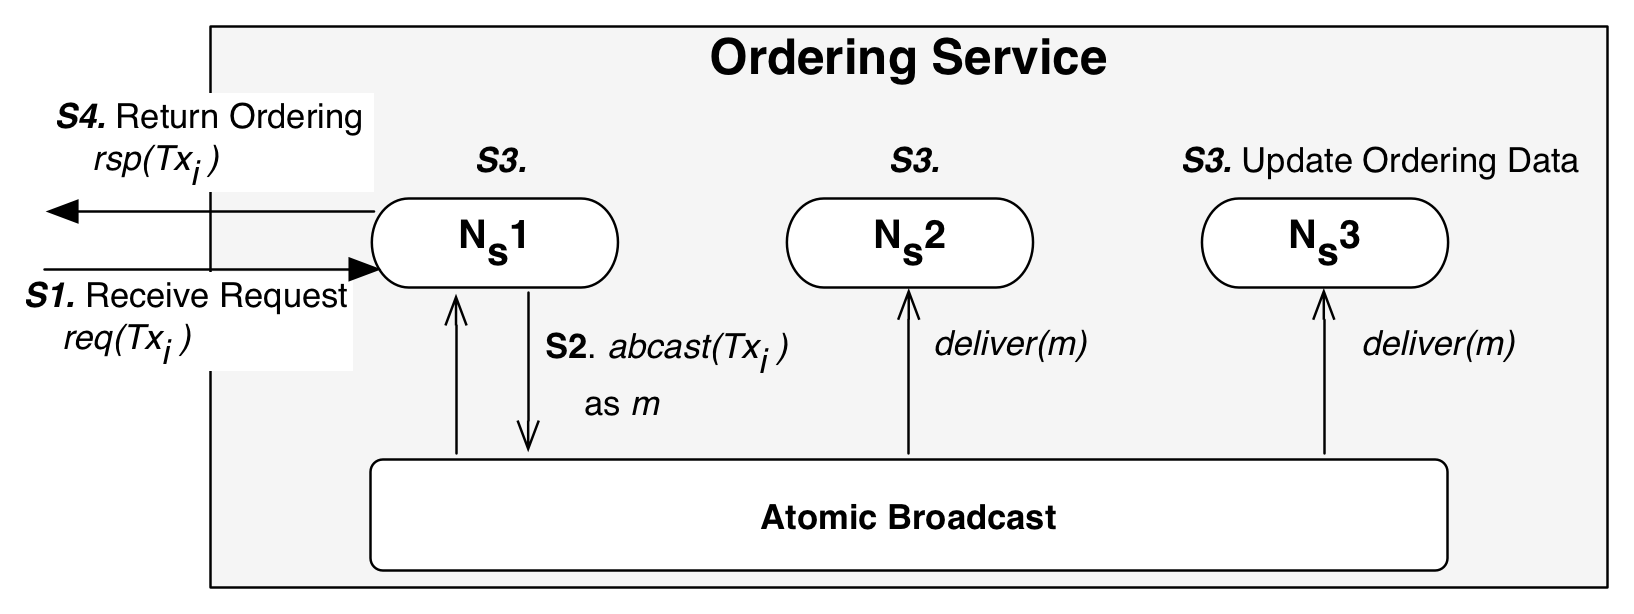
\includegraphics[width=1.0\textwidth]{scast_service}
         \caption[SCast Service Interactions]{SCast Service Interactions Diagram}
         \label{fig:scast_service}
    \end{figure}
    
    \subsection{Atomic Multicast Guarantees}
    The \textsf{SCast} protocol is a deterministic \emph{amcast} protocol, therefore for all \emph{amcast}s the protocol ensures that guarantees G1-G4, as stated in section \ref{sec:atomic_guarantees}, are met.      
    
    \subsection{Protocol Details} \label{ssec:scast_details}
    \subsubsection*{Client Nodes}
    \begin{description}
        \item[1. Delegate Backup Coordinator] \hfill \\
        For the purposes of fault-tolerance the first stage of the protocol is for $Tx_i.c$ to create a backup coordinator; where $Tx_i.c$ always denotes the original coordinator for transaction $Tx_i$.  $Tx_i.c$ selects any destination, $d$, $d \in Tx_i.dst$, and sends it the payload of the message ($prepare(Tx_i)$) that is to be multicast to $Tx_i.dst$.  $Tx_i.c$ then waits for an acknowledgement of receipt from $d$ before proceeding to stage 2 of the protocol.  If an acknowledgement is not received within a configurable amount of time, then $Tx_i.c$ simply selects another destination $d'$ from $Tx_i.dst$ and restarts the process.  
        
        The purpose of creating a backup transaction coordinator is to allow for the possibility that the $Tx_i.c$ may crash during the multicast process.  In the event of $Tx_i.c$ crashing, the group membership service for $c$-nodes detects the crash and the backup coordinator assumes responsibility for multicasting $prepare(Tx_i)$ to all $d \in Tx_i.dst - \{Tx_i.c\}$.  We denote the currently active transaction coordinator as $Tx_i.\tilde{c}$ and the original coordinator as $Tx_i.c$.  
        
        When $Tx_i.\tilde{c}$ takes over from the crash $Tx_i.c$, it completely restarts the multicast process and selects another node from $Tx_i.dst$ to be a backup coordinator.  In the unlikely event that the original coordinator and multiple backup coordinators crash, it is possible that there wont be a member of $Tx_i.dst$ left to utilise as a backup coordinator.  In which case a backup will not be created, as $Tx_i.\tilde{c}$ will be the last destination alive in $Tx_i.dst$, therefore if $Tx_i.\tilde{c}$ crashes the transaction is aborted by default.  
                
        \item[2. Request Ordering] \hfill \\
        Once a backup coordinator has been established, it is possible for the transaction coordinator to request a multicast ordering from the service.  \emph{Amcast}s are initiated by the $Tx_i.c$ randomly selecting a $s$-node, $N_s$, from the \emph{ordering service} and sending an \emph{amcast} request to that node - $req(Tx_i) -> N_s$; where $req(Tx_i)$ contains $Tx_i.dst$, $Tx_i.\tilde{c}$ and the unique id of the transaction, $Tx_i.id$.  Hence, $req(Tx_i) = \{Tx_i.id, Tx_i.dst, Tx_i.\tilde{c}\}$.  
        
        The content of the $prepare(Tx_i)$ message is not sent to $N_s$ as we only require a global order for $Tx_i$, therefore the contents of the message to be \emph{amcast} to $Tx_i.dst$ is irrelevant and including it would only increase bandwidth usage.  However, $req(Tx_i)$ must include $Tx_i.dst$ as this is the destination set of the \emph{amcast} that $Tx_i.c$ is trying to send, and the \emph{ordering service} needs this data to ensure that requirements CR1, CR2 and CR3 are satisfied.  
        
        \item[Waiting for a response from the \emph{ordering service} $\ldots$] \hfill \\
                If $Tx_i.\tilde{c}$ does not receive an ordering from the \emph{ordering service} after a specified timeout, then a different $s$-node, $N_s'$, is selected and the ordering request is resent - $req(Tx_i) -> N_s'$.
        
        \item[3. Receive Ordering] \hfill \\
        When $Tx_i.\tilde{c}$ receives $rsp(Tx_i)$ from $N_s$, it appends the ordering information to the original $prepare(Tx_i)$ message and multicasts $prepare(Tx_i)$ as $mcast(Tx_i)$ to all $Tx_i.dst$ including itself. 
        
        \item[4. Order Transaction] \hfill \\
        Upon receiving $mcast(Tx_i)$, a client node, $c$, will check the \emph{immediate} predecessor data contained within this message.  This data dictates which $mcast$ message should be delivered in the total order before $mcast(Tx_i)$.  For example, if the predecessor data dictates $mcast(Tx_i)$ is preceded by $mcast(Tx_h)$ at destination $d$, then $d$ cannot deliver $mcast(Tx_i)$ until it has delivered $mcast(Tx_h)$.  Hence, this data specifies the order in which transactions should be executed at a given $c$-node.  
        
        The predecessor data consists of a single multicast timestamp for each $d \in Tx.dst$, opposed to a list of past timestamps, in order to reduce the size of each $rsp$ message sent by the \emph{ordering service}.  The use of a single timestamp results in a cascading wait occurring if multiple message have not yet been received by $c$.  For example, if $c$ has received $mcast(Tx_j)$ but has not received its predecessors $mcast(Tx_h)$ and $mcast(Tx_i)$, $c$ will only be aware of $mcast(Tx_i)$ from $Tx_j$'s predecessor data.  However when $mcast(Tx_i)$ arrives, $c$ becomes aware that it has not yet received $mcast(Tx_h)$,  and will wait for $mcast(Tx_h)$ before delivering $mcast(Tx_i)$ and $mcast(Tx_j)$.          
    \end{description}

    \subsubsection*{Service Nodes}    
    \begin{description}
        \item[1. Receive Request] \hfill \\
            Upon receiving $req(Tx_i)$, an $s$-node places the request in its \emph{Abcast Request Pool} (ARP), which is a bounded queue for storing requests before they are \emph{abcast} to all $s$-nodes.  If an $s$-node's ARP becomes full, subsequent requests from $c$-nodes are rejected until space becomes available in the ARP.  When a $c$-node request is rejected a \emph{reject} response is sent to $Tx_i.c$.  If $Tx_i.c$ receives a \emph{reject} response from all $s$-nodes, then it can either abort $Tx_i$ or resend the \emph{amcast} request to another $s$-node after a configurable amount of time \footnote{This cycle will not continue indefinitely, as eventually the transaction will timeout and abort.}.  The ARP is necessary to ensure that if the \emph{ordering service} starts to become overloaded by client requests there is a \textquoteleft{}feedback' mechanism that makes $c$-nodes aware of the service's current limitations and allows clients to restrict user operations if necessary. 
            
        \item[2. Send Atomic Broadcast] \hfill \\
        A single thread, called the \emph{send} thread, is utilised for retrieving requests from the ARP and \emph{abcast}ing them to all $s$-nodes for ordering.  The \emph{send} thread retrieves an ordering request from the ARP and sends an \emph{abcast}, $m$, to all $s$-nodes containing the request.  Requests are retrieved from the ARP in the order that they were originally received (FIFO), however if no requests exist in the ARP then the \emph{send} thread waits for the pool to become non-empty before resuming \emph{abcast}ing.  
		
		All \emph{abcast} messages $m$, sent by an $s$-node, include the fields associated with $Tx_i$ which are sent as part of $req(Tx_i)$ \emph{i.e.}
		
		\begin{equation*}
			\begin{split}
			    m.tx\_id &= Tx_i.id \\
			    m.tx\_\tilde{c} &= Tx_i.\tilde{c} \\
	           m.dst &= Tx_i.dst
	        \end{split}
		\end{equation*}
		
		Furthermore, $m$ also includes the the address of the sending $s$-node and a sequence number, as $m.snid$ and $m.seq\#$, respectively.  Where $m.seq\#$ is an integer which is incremented by one every time an \emph{abcast} is sent §by this $s$-node.  
		
		\item[3. Update Ordering Data] \hfill \\    
		When an $s$-node, $N_s$, delivers an \emph{abcast} $m$ it checks its record to see if a request has already been processed for $m.tx\_id$.  If this is the first time that $N_s$ has encountered $m.tx\_id$, then $m$ is accepted and processed.  However, if $N_s$ has already processed a request for $m.tx\_id$ \footnote{Multiple client requests for $Tx_i$ can be \emph{abcast} between $s$-nodes as a consequence of $Tx_i.c$ crashing, or timing out, as these events result in $req(Tx_i)$ being sent multiple times.}, then it initiates the process detailed in section \ref{ssec:scast_fault_tolerance}.  %It is possible to discard a duplicate request as we know that all other $s$-nodes have, or will eventually, handle(d) the same version of a request as $N_s$ due to the guarantees provided by \emph{abcast}.  
		
        \paragraph{Assigning Total Order} \hfill \\
		Upon delivering and accepting $m$, $N_s$ assigns a global order to $m$ and the associated $m.tx_id$, which is represented as $m.order$.  
        
        \begin{equation*}
            m.order = ts\oplus m.seq\# \oplus m.snid
        \end{equation*}        		
		
        Where $\oplus$ is the append operator and $m.ts$ is the final timestamp provided by the underlying \emph{abcast} protocol that is utilised between $s$-nodes.  As $ts$ is generated by the underlying \emph{abcast} protocol and $m.seq\# \oplus m.snid$ is specified before broadcast, it is guaranteed that all $s$-nodes will produce the same $m.ts$.  
        
        \paragraph{Order definitions} \hfill \\
        The ordering of \emph{amcast} messages, and hence transaction ordering, is defined as follows.  We denote that an \emph{amcast} message $m$ precedes another \emph{amcast} $m'$ in the global total order, \emph{i.e. $m.order < m'.order$} as  \scalebox{1.5}{$m \prec m'$} and define this relationship as:
        \begin{equation*}
            \begin{split}
                   m \prec m' &\implies  m.ts < m.ts \\
                   & \lor \left(m.ts = m'.ts  \land m.seq\# < m'.seq\#\right)
            \end{split}
        \end{equation*}
        
        Furthermore, we state that $m$, \emph{immediately} precedes $m'$ in the total order if the following statements are true:
        
        \begin{enumerate}[label={(\roman*)}, leftmargin=5em]
            \item    $m \prec m'$
            \item    There is no $m'' : m \prec m'' \prec m'$
        \end{enumerate}

        and we denotes this relationship as \scalebox{1.5}{$\quad m \llcurly m'$}.  
        
        As \textsf{SCast} is an \emph{amcast} protocol, it is possible for each $m$ to have a different destination set.  Consequently, a message's ordering also needs to be defined relative to the other messages that have been received by each $d \in m.dst$.  Therefore, let \emph{amcast} $\tilde{m}$ precede $m$ for any destination $d$, if:
        
        \begin{equation*}
            d \in \tilde{m}.dst \cap m.dst : \tilde{m} \prec m
        \end{equation*}
        
        and we denote this relationship as  \scalebox{1.5}{$\quad \tilde{m} \prec_d m$}.  
        
        %\textbf{Note: } $\tilde{m} \prec_d m \implies  \tilde{m} \llcurly m$, however $\tilde{m} \llcurly m \centernot\implies \tilde{m} \prec_d m$.  For example, consider $m_i$ and $m_j$, if $m_i \prec m_j$ but $m_i.dst \cap m_j.dst = \{\}$ then it is not possible for $m_i$ to precede $m_j$ at any $d \in m_i.dst$.  
        
        Finally, we state that an \emph{amcast}, $\tilde{m}$, \emph{immediately} precedes $m$, with respect to destination $d$, if:

        \begin{enumerate}[label={(\roman*)}, leftmargin=5em]
            \item    $\tilde{m} \prec_d m$
            \item    There is no $m' : \tilde{m} \prec_d m' \prec_d m$
        \end{enumerate}
        
        and we denote this relationship as \scalebox{1.5}{$\quad \tilde{m} \llcurly_d m$}.  
        
        \paragraph{Recording Transaction Ordering} \hfill \\
        Once an order has been associated with $Tx_i$, it is necessary for a $s$-node to update its history of transaction orderings to include $Tx_i$.  
        
		Once a request has been accepted, its transaction $Tx_i$ is associated with a global timestamp $ts$: $req(Tx_i).ts = m.ts\oplus m.o$; where $\oplus$ is the append operator and $m.ts$ is the final timestamp provided by the underlying \emph{abcast} protocol utilised between $s$-nodes.  As the global timestamp is generated by the underlying \emph{abcast} protocol, it is guaranteed that all $s$-nodes will assign the same $ts$ to each transaction.  Once a global timestamp has been allocated to $Tx_i$ it is necessary for the $s$-nodes transaction history to be updated.  We refer to this transaction history as the \emph{immediate predecessor} data, as we simply store the last calculated $ts$ of a transaction that involves each client node.  For example, if a $c$-node $c$ was last involved in a transaction $Tx_i$, then the \emph{immediate predecessor} data would state that the last transaction involving node $c$ was $Tx_i$.  The transaction assigned to $c$ will continue to be $Tx_i$ until a new ordering request that involves $c$ is received by the ordering service.  
		
		The storage of \emph{immediate} predecessor data works as follows: All $s$-nodes maintain a transaction history as an associative array that maps a $c$-node address to the id of the last transaction they were associated with, hence its \emph{immediate} predecessor.  So for each ordering request, the global timestamp assigned to the request is associated with each of the $c$-node addresses that participate in the transaction.  %When a $s$-node delivers an \emph{abcast} $m$, it knows that all other $s$-nodes have delivered, or will deliver, $m$ in the same order.  Therefore, when $m$ is processed by an $s$-node, it is guaranteed that all other $s$-nodes will have processed $m$ in the exact same order, hence we know that the transaction history is consistent across all $s$-nodes.  
		
		For example, consider an ordering request for a transaction $Tx_i$ that has a destination set $Tx_i.dst = {N_c1, N_c2}$.  When an $s$-node processes $req(Tx_i)$ after it has been \emph{abcast}, it will update its predecessor data so that the entry for $N_c1$ and $N_c2$ equals $Tx_i$.  Now consider that another ordering request is processed for a transaction $Tx_j$ that has a destination set $Tx_j.dst = {N_c1, N_c3}$.  The predecessor data will show that the last transaction associated with $N_c1$ and $N_c3$ is $Tx_j$, whereas the last transaction associated with $N_c2$ is $Tx_i$.  This scenario is visualised in figure \ref{fig:predecessor_data}, with the right most transaction linked to a $c$-node representing the latest transaction in the global order that involved this address.  
		
        \begin{figure}[htbp!] 
        \centering    
         \includegraphics[width=.60\textwidth]{predecessor_data}
         \caption[Transaction Predecessor Data]{Transaction Predecessor Data}
         \label{fig:predecessor_data}
    \end{figure}
		
		Note that the immediate predecessor of $Tx_i$ is applicable to \emph{all} transactions involving a given $d$ - not just those that originate from $Tx_i.c$ nor just those that are handled by one $s$-node. Thus, it is specific to each $d \in Tx_i.dst$ and ensures that delivery at every $d$ is per the finalized $Tx_i.ts$.  To illustrate this, let $Tx_i.c$ submit $req(Tx_i)$ to $N_s$, $Tx_j.c$ submit $req(Tx_j)$ to $N_{s'}$ and $d \in Tx_i.dst \cap Tx_j.dst$. Say, the ordering service places $req(Tx_j)$ before $req(Tx_i)$ in the total order, if $d$ receives $Tx_i$ before $Tx_j$, it cannot deliver $Tx_i$ until it delivers $Tx_j$.
		
        \item[4. Return Ordering] \hfill \\
		Once the local $s$-node, $N_s$, has assigned a timestamp to a transaction and updated its transaction history, it is possible for a response message to be sent to the transaction coordinator.  However, as all $s$-nodes will receive, and assign the same timestamp to each request, it is necessary for a single $s$-node to take responsibility for sending the response message.  This is achieved by utilising the $m.o$ field set in stage 2 of the service protocol: If $N_s = m.o$ then $N_s$ is the $s$-node that initially received $req(Tx_i)$, therefore $N_s$ takes responsibility for sending a response message.  
				
		A response message, $rsp(Tx_i)$ consists of two types of ordering data: the timestamp agreed by $s$-nodes for $Tx_i$, and the timestamps of $Tx_i$'s \emph{immediate} predecessors.  The latter is the timestamps of all transactions that directly precede $Tx_i$.  More precisely, for all destinations $d \in Tx_i.dst$, the timestamp of the transaction which appears before $Tx_i$ in the global order is specified, so that no $d$ can miss a transaction in the global ordering.  Hence, the timestamps returned to the client nodes are the timestamps that were overwritten by the current transaction $Tx_i$ when the predecessor data was updated.  
		
		For the purpose of fault-tolerance, each $s$-node also maintains a short history of the response headers that are generated for each ordering request.  This enables past orderings to be returned to $c$-nodes in the event of the original transaction coordinator crashing.  
    \end{description}

	\subsection{Fault-Tolerance: Node Crashes}\label{ssec:scast_fault_tolerance}
	Fault-tolerance in \textsf{SCast} must consider the consequences of both crashed $c$-nodes and $s$-nodes.  Here we explore the consequences of both $c$-node and $s$-node crashes during various stages of a \textsf{SCast} \emph{amcast}.  For the sake of simplicity, we only consider node crashes from the perspective of a single transaction, however it is worth noting that each $c$-node would typically have multiple transactions executing concurrently.  
	
    \subsubsection*{Client Node Crash}
	\begin{description}
         \item[\emph{Local Tx Execution}]  \hfill \\
         If a $c$-node, $Tx_i.c$, crashes during or directly after the local execution of a transaction, $Tx_i$, then no action needs to be taken as no interactions with other $c$-nodes or $s$-nodes have occurred.  
		
		\item[\emph{Stage 1}]  \hfill \\
		If $Tx_i.c$ crashes during the creation of a backup coordinator then two scenarios are possible:
		    \begin{itemize}
			    \item    The backup coordinator never receives the $prepare(Tx_i)$ message, in which case the transaction  can only be aborted as its contents have been lost.  
			    \item    The backup coordinator successfully receives the $prepare(Tx_i)$ message and attempts to acknowledge the original coordinator.  The original coordinator will never receive the acknowledgement as it has crashed; however, the backup coordinator will still restart the multicasting process from stage 1 of the protocol. The backup coordinator takes over from the original coordinator as soon as the group membership protocol has detected the crash and issued a new view to the client nodes.  
		    \end{itemize}     
		    
		\item[\emph{Stage 2}]  \hfill \\
        If $Tx_i.c$ crashes before or during the sending of a request $r$ to the ordering service, then the backup coordinator simply restarts the multicast process when the GM service recognises that $Tx_i.c$ has crashed.  It is possible that the $s$-node that $r$ was sent to, $N_s$, will still receive $r$, in which case $r$ will be processed as normal by the $s$-node.  When the backup coordinator sends a new ordering request to the service for $Tx_i$, $r'$, this request is also processed.  The ordering service accepts the request which is delivered first by the \emph{abcast} protocol and sends a response to the transaction coordinator specified in the accepted request.  Assuming that both coordinators send $r$ and $r'$ to $N_s$: If the $s$-nodes deliver $r$ first in the total order, then a response is  sent to the original coordinator of $Tx_i$ as $N_s$ is unaware that this $c$-node has crashed.  However, when $N_s$ delivers $r'$ it deduces that both $r$ and $r'$ concern $Tx_i$ and that $r'$ will only have been issued if the original coordinator had crashed, therefore $N_s$ resends the original $rsp(Tx_i)$ message to the coordinator of $r'$.  Similarly, it is possible that $r'$ is sent to a different $s$-node than $r$, $N_s'$, in which case $N_s'$ will also resend the original $rsp(Tx_i)$ message, as $N_s'$ must have received both $r$ and $r'$ as per the guarantees of \emph{abcast}.  
        
        In addition to the various scenarios described above, it is also possible that $r$ was never received, in which case the $s$-node that received $r'$ will send a response message to the coordinator of $r'$ as if it were a normal request.  
        
        \item[\emph{Stage 3}]  \hfill \\
        If $Tx_i.c$ crashes before receiving a response from the ordering service, then the backup coordinator takes over and restarts the multicast process.  When the backup coordinators request is received by an $s$-node, the $s$-node checks its recent history of processed requests and returns the ordering data assigned to this transaction.  The size of the recent history stored by the service should be configurable to allow for varying levels of resilience.   This is because as the size of the past history increases, the chances of a prior transaction ordering being discarded decreases.  Thus a larger record provides a greater level of fault-tolerance, but at the expense of utilising more system resources.  
        
        \item[\emph{Stage 4}]  \hfill \\
        If $Tx_i.c$ crashes before the multicasting of $mcast(Tx_i)$ to all $d \in Tx_i.dst$ has finished, then two scenarios are possible:
           \begin{itemize}
			    \item    The backup coordinator has received $mcast(Tx_i)$ from $Tx_i.c$, in which case the backup coordinator can simply restart the multicasting process (Stage 4).
			    \item    The backup coordinator has not received $mcast(Tx_i)$ from $Tx_i.c$, in which case the protocol must be restarted.  
		    \end{itemize}  
    \end{description}
    
	\subsubsection*{Service Node Crash}
	\begin{description}
       \item[\emph{Stage 1-3}] \hfill \\
       If a $s$-node crashes while a $Tx_i.c$ is issuing a service request, then the request will simply timeout and the $Tx_i.c$ will resend the request to another $s$-node.  Its possible that the request was \emph{abcast} to other $s$-nodes before the crash, in which case the other $s$-nodes will process the request and simply return the established ordering for a transaction when subsequent requests are received from the transaction coordinator.  
    \end{description}
    
    \subsection{Fault Tolerance: Split Brain}
    Split brain refers to a situation whereby the current view of a group of processes has been partitioned into two or more views, which is usually caused by one or more failures occurring at the underlying network layer. Typically, these views will be consist of disjoint sets of processes, however it is possible for overlapping to occur between multiple views.  Eric Brewer's seminal CAP theorem, states that it is impossible for a system to provide Consistency, Availability and Partition Tolerance simultaneously \citep{Brewer:2000:TRD:343477.343502,6133253, Gilbert:2002:BCF:564585.564601}.  Therefore, when designing a solution for handling split brain scenarios, which is a partition by definition, it is necessary for either availability or consistency of part of the system to be compromised.  
    
    Handling split brain partitions across a cluster of $c$-nodes in which \textsf{SCast} operates is ultimately the responsibility of the applications using \textsf{SCast} for \emph{amcast}s.  For example, in the case of Infinispan, if a cluster of $c$-nodes is partitioned then it is the responsibility of Infinispan to determine whether consistency or availability should be preserved.  However, as a Infinispan cluster will be dependent on \textsf{SCast} and its \emph{ordering service}, it is necessary for such a service to provide a strategy for handling partitions that occur within the service itself.  
    
    Our solution for handling partitions within an \textsf{SCast} ordering service is to utilise a majority partition scheme.  When a network partition occurs, the $s$-nodes whose new network view is a majority of the previous view continues to accept client requests and operate as an \emph{ordering service}.  Whereas the $s$-nodes who are now in the minority partition sacrifice availability by rejecting future client requests until the juncture of the two partitions.  The $s$-nodes in the minority partition reject client requests in order to allow for the consistency of the system to be readily resolved when the two partitions are rejoined.  For example, if the availability of the minority partition was not sacrificed, the merging of state required when the two partitions are rejoined would not be trivial, with the predecessor data and active client requests of each partition having to be fused in a way that does not compromise \emph{amcast} guarantees G1-G4.  Whereas, when only one partition remains active when the network is divided, it is possible for the $s$-nodes in the minority partition to clone the state of an $s$-node from the majority partition and start accepting client requests again.  
    
    The majority partition scheme detailed above works as expected when $|s$-nodes$|$ is an odd number, however if it is an even number, then it is possible for the \emph{ordering service} to be partitioned so that no majority partition exists.  To avoid such a scenario it is necessary for a \textquoteleft{}watcher' node to be utilised when $|s$-nodes$|$ is even.  A watcher node does not participate in the \textsf{SCast} protocol, rather it is used purely for tie-breaking between the views of two $s$-node partitions that would otherwise be equal.  

\section{Message Bundling}\label{ssec:abaas_optimisations}
		When utilising \textsf{AmaaS} it is possible for all \emph{amcast} requests received from $c$-nodes to be bundled into a single \emph{abcast} (between $s$-nodes) at a receiving $s$-node, regardless of their destination set.  This is because $s$-nodes are only required to send \emph{abcast}s to other $s$-nodes in order for a consensus on transaction ordering to be reached, therefore the destination set for each \emph{abcast} is the same for all $c$-node requests.   The ability to bundle multiple \emph{amcast} requests into a single \emph{abcast} reduces the number of times that consensus needs to be reached between all $s$-nodes.  Thus further reducing the number of $N->1$ communication steps required, with the total number of \emph{abcast}s reduced by $\left\vert bundle \right\vert$; where $bundle$ is the number of  \emph{amcast} requests from $c$-nodes that are sent as a single \emph{abcast}.  As a result of this optimisation network traffic is significantly reduced when requests are frequent, resulting in the capacity and scalability of an \emph{AmaaS} service increasing. Conversely, message bundling does not compromise performance when the number of service requests is low, as bundling does not require any intensive computation or additional communication steps.  
    
    In the case of \textsf{SCast}, message bundling can be implemented as follows: The \emph{send} thread retrieves ordering requests from the ARP in their arrival order, and bundles them into a single message bundle $mb$, with the first message being stored at index 0 and so on.  This message bundle is then \emph{abcast}as a single $m$ to all $s$-nodes.  A configurable upper limit can be placed on the maximum size of a bundle message. \footnote{The maximum size could be specified in terms of bytes or the number of messages to be bundled.} If this upper limit is reached and the ARP still has available requests, then the \emph{send} thread will start processing the next message bundle, $mb'$, once $m$ has been \emph{abcast}.  
    
    Upon receiving $m$, each $s$-node must \emph{unbundle} $mb$ and process each individual $c$-node request in the same manner as if the request had been \emph{abcast} as a single request.  A consequence of multiple ordering requests being bundled in to a single \emph{abcast} is that the timestamps utilised in \textsf{SCast} to uniquely order transactions are no longer valid, due to multiple transactions being associated with a single $m$, and hence a single $m.ts$.  Therefore, in order to uniquely order a transaction $Tx_i$, within $mb$, we define the unique timestamp of each request as $ts$: $req(Tx_i).ts = m.ts\oplus m.o \oplus$\emph{sequence number} of $req(Tx_i)$ within $mb$.  

\section{Limitations of Existing Coordination Services}\label{sec:limitations_existing_coordination}
It is possible to utilise existing coordination solutions ($\S$ \ref{sec:coordination}), such as Zookeeper\citep{Hunt:2010:ZWC:1855840.1855851} and Chubby\citep{Burrows:2006:CLS:1298455.1298487}, as the basis of a \textsf{AmaaS} service.  However, both of these solutions are intended for high levels of read requests, not workloads that consist predominantly of write operations; where a write operation is any client operation that changes the state of a single $s$-node, therefore requiring the state of all other $s$-nodes be updated in order to maintain a consistent state machine.  

Write operations are vital to the \textsf{AmaaS} model, as every ordering request from a $c$-node requires an update to an $s$-node's transaction history and hence requires a consensus to be reached between $s$-nodes.  Both Zookeeper and Chubby propagate write operations by utilising a quorum based \emph{abcast} protocol to reach consensus.  Consequently, all write operations are coordinated by a single master node, and as a result the throughput of such a service is always be limited by the capabilities of the elected master node.  For example, the Chubby service utilises an implementation of the Paxos protocol to coordinate write operations.  However, the performance of paxos and its variants have been shown to be unpredictable under even mild levels of stress, with sustained periods of demand preventing a consensus being reached \citep{DBLP:journals/corr/MarandiBPB14}.  Therefore, if either of the Quorum based implementations Zookeeper or Chubby were utilised as the basis of an \textsf{AmaaS} service, the service's performance would be poor due to the larger number of write operations required.  

\section{A New Atomic Broadcast Solution is Required}
Existing \emph{abcast} and \emph{amcast} solutions are of two types ($\S$ \ref{sec:atomic_guarantees}); quorum-based and GM based.  GM based protocols provide the lowest latency message delivery in the absence of node crashes, but at the expense of blocking when node crashes do occur.  This blocking behaviour is acceptable when such protocols are utilised in traditional P2P environments like Infinispan, as it is presumed that the blocking will only occur at a small subset of nodes in the cluster.  In which case system \emph{liveness} is maintained by the majority of nodes in the cluster.  However in the \textsf{AmaaS} model, if a $s$-node utilises a GM protocol for \emph{abcast}ing requests amongst all $s$-nodes and a single $s$-node crashes, all $s$-nodes will block, resulting in no client requests being satisfied. This means that, not only are the $s$-nodes participating in the \emph{abcast} blocked, but as a consequence of this blocking, so to are all of the $c$-nodes utilising the service.  Therefore the entire system's \emph{liveness} is lost until the GM protocol is able to detect the $s$-node crash and unblock the ordering service.  

Alternatively, a quorum-based protocol, such as those detailed in \ref{sec:coordination}, can be utilised between $s$-nodes.  Such protocols perform worse than GM protocols in the absence of node failures ($\S$ \ref{sec:limitations_existing_coordination}), however they only block mildly when a leader node crashes or is falsely suspected of crashing.  

In order to maximise the effectiveness of the \textsf{AmaaS} system model, a new \emph{abcast} protocol is required.  This protocol must provide non-blocking message delivery in the presence of node failures, whilst allowing for low-latency, high-throughput \emph{abcast}s in their absence.  

\section{Summary}
This chapter presented \textsf{AmaaS} - a new model for \emph{amcast} protocols that utilises a dedicated set of nodes to provide \emph{amcast} as a service to distributed transactional systems.  We then presented a new protocol \textsf{SCast} that provides fault-tolerant \emph{amcast}ing in such an environment.  Lastly, we outlined the shortcomings of existing \emph{abcast} solutions and the need for a new protocol in order for the \textsf{AmaaS} approach to be fully realised. 